\title{Computational Neurophysiology - Assignment 2}
\author{Ryan Spangler}
\date{\today}

\documentclass[12pt]{article}

\usepackage{commath}
\usepackage{graphicx}

\setcounter{secnumdepth}{0}

\begin{document}
\maketitle

\section{1 - Cable Equation}

\emph{Modeling the neuronal membrane and axon as a one-dimensional cable yields the second-order partial differential equation discussed in class (with passive currents only):}

$$ \lambda^2\pd[2]{V}{x}-\tau\pd{V}{t}-V=0 $$

\vspace{6pt}

\emph{a.  Explain, with reference to appropriate membrane (transversal) and intracellular (longitudinal) resistances and capacitances, what $\lambda$ and $\tau$ are.}

\vspace{10pt}

$\lambda$ and $\tau$ are the spatial and temporal factors of the membrane potential respectively.  Each governs the order with which the space and time quantities of the membrane potential vary.  

$\lambda$ is known as the ``electrotonic length'', which incorporates the longitudinal resistance and membrane resistance of the cell into a measure of how far current spreads in the given cable.  The higher $\lambda$, the more widespread are the effects of any given current spatially throughout the cell.  Its official form is:

$$ \lambda=\sqrt{\frac{ar_m}{2r_L}} $$

Electrotonic length is in units of length, as the two resistance terms cancel out, leaving only the area term in length squared, which is subsequently rooted.  As can be seen, if the membrane resistance grows, so does the electrotonic length, since less current will be flowing through the membrane and therefore focused into the longitudinal direction.  Conversely, a rise in intracellular resistance will reduce the electrotonic length, as it takes more voltage to reach the same distance as before.

$\tau$ is the temporal order of the change in membrane potential.  It is relative to both the membrane resistance and membrane capacitance.  

$$ \tau=c_mr_m $$

This follows, as the greater the capacitance of the membrane the swifter its voltage will change.  Also, the higher the resistance of the membrane the more current will be flowing through the intracellular volume.

\vspace{10pt}

\emph{b.  What would be the effect of a greatly increased membrane resistance on propagation of the action potential along the axon? What would it mean in terms of the equation?}

\vspace{10pt}

The higher the membrane resistance, the less current is leaking out of the cell and the more that is focused towards traveling down the axon.  In the equation, both $\lambda$ and $\tau$ grow in the presence of rising membrane resistance, meaning all change in potential (temporal and spatial) is happening more quickly and over a wider area.

\vspace{10pt}

\emph{c.  i.  What is the stationary solution of the cable equation? (i.e. what happens if you set $\pd{V}{t} = 0$)?  How would you interpret this result in terms of what is happening in the neuron?}

\vspace{10pt}

If we were to set $\tau=0$ and erase all temporal activity, the cable equation becomes:

$$ \lambda^2\pd[2]{V}{x}-V(x)=0 $$

with a solution of:

$$ V(x)=e^{\frac{-x}{\lambda}} $$

In this case, only the spatial behavior (represented by x) is present.  The membrane potential is held constant, degrading exponentially along the length of the axon inversely proportional to the electrotonic length.  This would come about in the absence of any stimulus or current from an earlier neuronal section.

\vspace{10pt}

\emph{    ii.  What happens if you ignore spatial diffusion? What does this represent in terms of the biophysics of the neuron?}

\vspace{10pt}

If you ignore spatial diffusion, by setting the electrotonic length to zero for example, you have essentially a single compartment model with only passive membrane dynamics.  

$$ -\tau\pd{V}{t}-V(t)=0 $$

\vspace{4pt}

and solving with respect to t:

$$ V(t)=e^{\frac{-t}{\tau}} $$

This equation tells us the voltage will leak from the cell inversely proportional to both the membrane capacitance and resistance.  Which follows, since the higher the resistance the slower the potential will decay, and the higher the capacitance the longer it will take for the voltage to completely diffuse.

\section{2 - Transient Calcium Channels}

\emph{The cell sketched below contains T-type $Ca^{++}$ channels, $K_{Ca}$ channels, and leak channels.} 

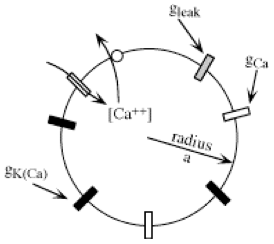
\includegraphics[scale=0.7]{transientcalcium.png}

\emph{The conductance of the $K_{Ca}$ channels is determined by the intracellular Ca++ concentration according to the following equation:}

$$ g_{K_{Ca}}=\overline{g}_{K_{Ca}}\frac{[Ca^{++}]}{K_{Ca}+[Ca^{++}]} $$

\emph{a.  Write the differential equations necessary to model this system. Clearly define the state variables of the system. For simplicity, assume a single $[Ca^{++}]$ state, which is the average calcium concentration in the cell.}

\vspace{10pt}

For a membrane containing only transient calcium channels and calcium-activated potassium channels (along with leak-current and a point stimulus for good measure), the set of equations defining the system would be:

$$ C\od{V}{t}=I-\overline{g}_Tr^3s(V-E_T)-g_{K_{Ca}}n(V,[Ca^{++}]_i)(V-E_K)-g_L(V-E_L) $$

In this equation, the first term on the left side is the stimulus current, next is the transient calcium current, the calcium-activated potassium current, and finally the leakage current.  

In the transient calcium current there are two state variables, r and s.  r is raised to the third power and represents the onset of the calcium current.  s is the inactivation term, which counteracts the action of the channel if brought to zero.

The calcium-activated potassium current has only one state variable, n, which depends on both the voltage and the calcium concentration.  

The equation for the concentration of calcium inside the cell is:

$$ \od{[Ca^{++}]_i}{t}=\frac{1}{\tau_{Ca}}([Ca^{++}]_{\infty}-[Ca^{++}]_i) $$

This represents a continuous transport of calcium out of the cell, relative to the level at which it is currently at.  This serves to maintain a level of calcium in the intracellular space in the absence of other calcium activity.  

The other state variables have associated functions:

$$ \od{r}{t}=\alpha_r(V)(1-r)-\beta_r(V)r $$
$$ \od{s}{t}=\alpha_s(V)(1-s)-\beta_s(V)s $$
$$ \od{n}{t}=\alpha_n(V,[Ca^{++}]_i)(1-n)-\beta_n(V,[Ca^{++}]_i)n $$

You will notice that the state variable n depends on both the voltage and the calcium concentration inside the cell, whereas the other two r and s are vanilla gates depending only on membrane potential.

\vspace{10pt}

\emph{b.  Write the equations for the steady-state, or resting state, for the cell modeled in part a). Make sure you have enough equations to specify the resting values of all the state variables.}

\vspace{10pt}



\vspace{10pt}

\emph{c.  Add these currents to the Neuron code for the single compartment Hodgkin-Huxley model used in Assignment 1. Discuss the changes in the spiking behavior of the neuron as you increase the maximum conductances of the T-type $Ca^{++}$ currents and $K_{Ca}$ currents.}

\vspace{10pt}

\end{document}
